
\subsection{Term unfolding for homogeneous inputs}
\label{sec:homo-unfold}

\subsubsection{Preliminaries}

\paragraph*{Error raising.} We can think of the type $\ranked{1}$ as an error type. Indeed, the following raising error functions are derivable.
\begin{lemma}\label{lem:error-raising}
Let $\rSigma$ and $\rGamma$ be two datatypes. The functions
$$\begin{array}{rll}
\ranked{\tmonad(\Sigma+1)} &\ranked{\to }&\ranked{\tmonad \Sigma +1}\\
\ranked{(\Sigma+1) \otimes (\Gamma+1)} &\ranked{\to} &\ranked{\Sigma\otimes \Gamma+1 }\\
\ranked{\shallowterm {(\Sigma+1)}{(\Gamma+1)}} &\ranked{\to} &\ranked{\shallowterm\Sigma\Gamma +1}\\
\ranked{\reduce k (\Sigma+1)} &\ranked{\to} &\ranked{\reduce k \Sigma +1} 
\end{array}$$
which are defined as follows
\begin{align*}
 t \text{ of arity } n \ \ \mapsto \  \begin{cases}
    t & 
    \text{if $t$ does not contain any element of $\ranked{1}$,}\\
    n & \text{otherwise.}
\end{cases}
\end{align*} are derivable.
\end{lemma}
These functions can be easily derived using Proposition~\ref{prop:forat} and distributivity prime functions. The details of the proof are left as an exercise to the reader.
 
\paragraph*{Partial functions.} Thinking of $\ranked{1}$ as an error datatype, a function of type $\ranked{\Sigma \to \Gamma +1}$
can be seen as a partial function from $\rSigma$ to $\rGamma$. We write 
\begin{align*}
\ranked{\Sigma\rightharpoonup \Gamma}
\end{align*}
as a notation for the function type $\ranked{\Sigma \to \Gamma +1}$.  
Using the error raising mechanisms discussed earlier, we can manipulate transparently partial function. Indeed, all datatype constructors can be lifted to partial functions, by composing the liftings (1)--(4) with the error raising functions from Lemma~\ref{lem:error-raising}. For example, if $\ranked{f:\Sigma\rightharpoonup \Gamma}$ is a partial function, then $\ranked{\tmonad f:\tmonad\Sigma\rightharpoonup \tmonad\Gamma}$ is defined as the composition
\begin{align*}
\ranked{\tmonad\Sigma\xrightarrow{\tmonad f} \tmonad(\Gamma+1) \xrightarrow{\text{Error raising}} \tmonad \Gamma +1}.
\end{align*}


\paragraph*{Partial shallow unfold}
 If $\rGamma$ and $\rDelta$ are types, we define $\ranked{\Gamma\odot\Delta}$ to be $\ranked{\Gamma.(\set{1}+\Delta)}$. We call its inhabitants the \emph{partial shallow} terms. A partial shallow term looks like this
\begin{center}
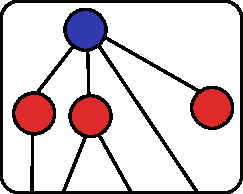
\includegraphics[scale=.4]{partial-shallow-term.pdf}
\end{center}
We define the \emph{partial shallow unfolding} function as the extension  of the shallow unfold function of Figure~\ref{fig:weak-unfolding} to partial shallow terms. It is the function of type 
\begin{align*}
\ranked{{\reduce k \Sigma}\odot{\Gamma^k} \to \reduce k ({\Sigma}\odot{\Gamma})} 
\end{align*}
defined as in the following picture
 \begin{center}
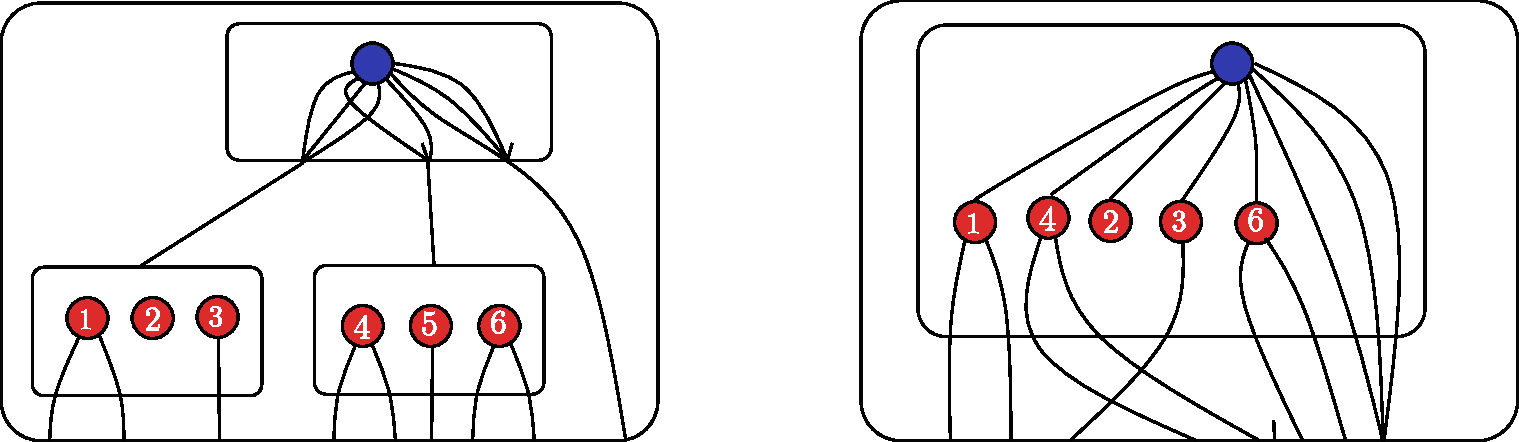
\includegraphics[scale=.4]{partial-shallow-unfold.pdf}
 \end{center}


\subsubsection{Term unfolding for constant-twist inputs}

We say that a term $ t \in \tmonad \mati k \rSigma$ is a \emph{constant-twist term}  if each twist of an internal branches is a constant function. Note that the internal twists need not to be the same constant function. Here is an example of a constant-twist term

  \begin{center}
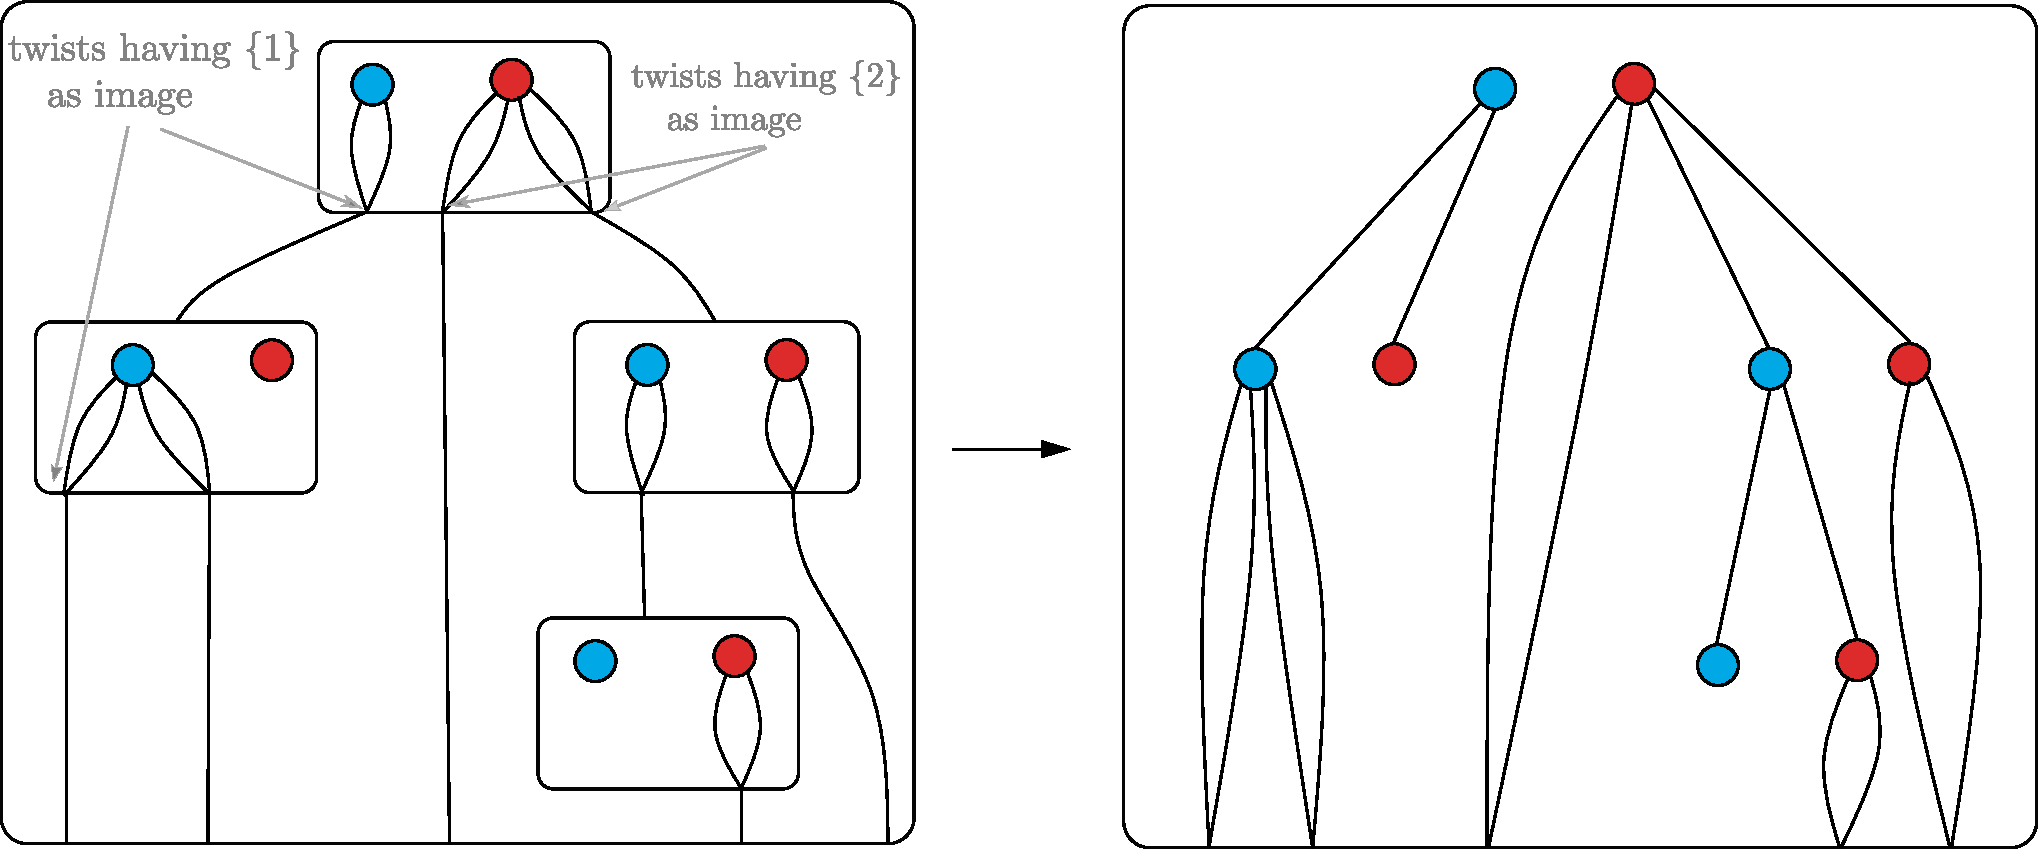
\includegraphics[scale=.4]{one-unfold.pdf}
 \end{center}
 This section is devoted to proving the following lemma. 

\begin{lemma}\label{lem:homo-twist}
    Let $k \in \set{1,2,\ldots}$. There is a derivable operation 
    \begin{align*}
        \ranked{f : \tmonad \mati k \rSigma \to \mati k {(\tmonad \Sigma)} }
        \end{align*}      
which coincides with unfolding for all constant-twist inputs.
\end{lemma}

\begin{proof}
The function $f$ can be implemented by a derivable function, which we construct using following steps. We use the example above as a running example to illustrate our construction.
\begin{itemize}
 \item We start by unfolding the external twits using the corresponding basic function. We get a term in $\ranked{\reduce k \tmonad \Sigma^{[k]}}$. Our example becomes like this
   \begin{center}
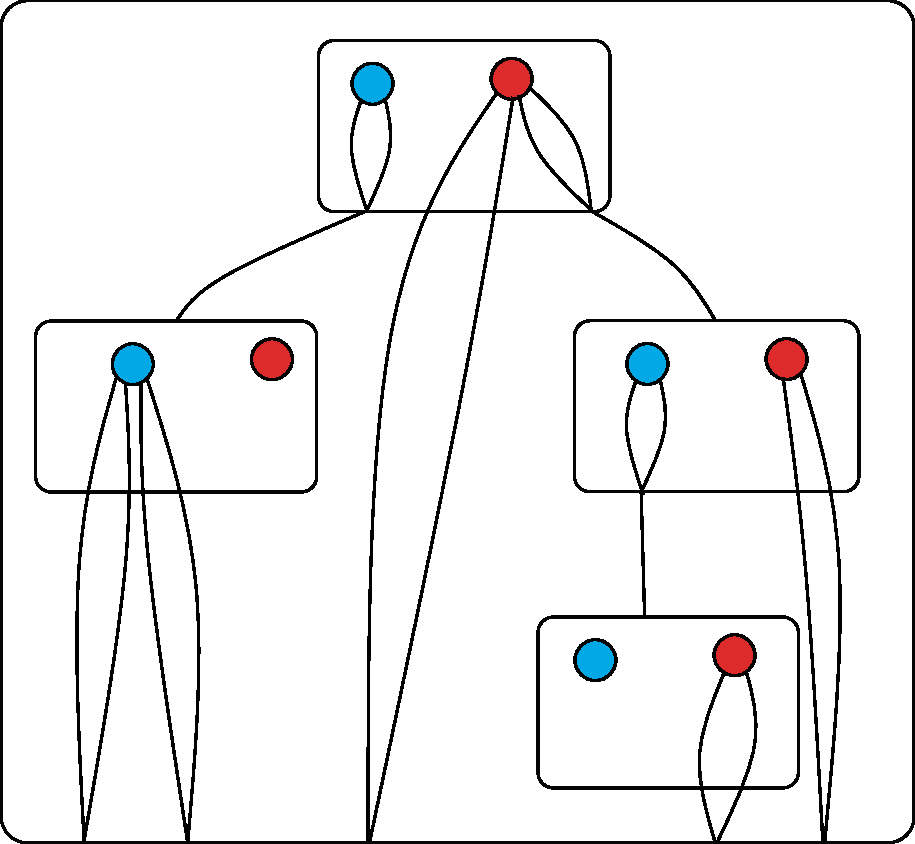
\includegraphics[scale=.4]{one-unfold1.pdf}
 \end{center}
 \item Next, we will transform each matrix power node into a tensor product as follows 
 \begin{align*}
 \ranked{ \Sigma^{[k]} \rightarrow \reduce k (\reduce k \Sigma \otimes \dots \reduce k \Sigma) \to \reduce 1 (\reduce k \Sigma)^k}
 \end{align*}
 The idea here is that, since the image of each twist is a singleton,  the ports of the matrix power are independent. We can then transform safely each node into a tensor product. After that, we transform each tensor product $\ranked{(\reduce k \Sigma)^k}$ into a shallow term $\ranked{k.\reduce k \Sigma}$ which we see itself as a term of type $\ranked{\tmonad(k+\reduce k\Sigma)}$. After the application of the unfolding function $\mathrm{unfold}_1$ followed by a flattening, and the simplification of $\ranked{\reduce k \reduce 1 \tmonad (k+\reduce k \Sigma)}$ into $\ranked{\reduce k \tmonad (k+\reduce k \Sigma)}$ we get a term in $\ranked{\reduce k \tmonad(k+\reduce k \Sigma)}$. Our running example becomes as follows after this step
   \begin{center}
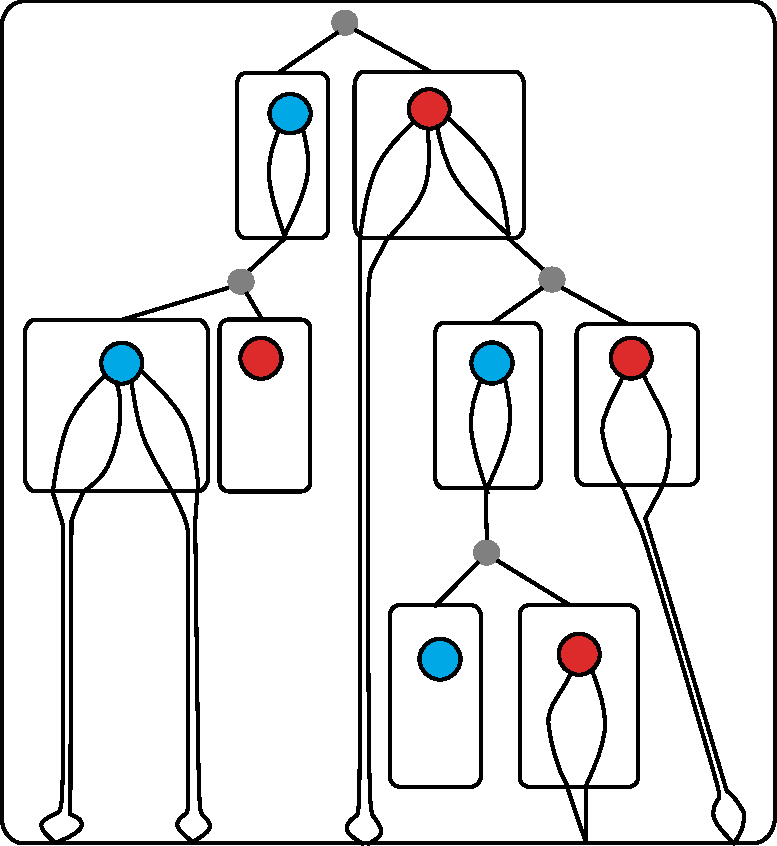
\includegraphics[scale=.4]{one-unfold2.pdf}
 \end{center}
 \item Now we apply the factorization 
 \begin{align*}
 \ranked{\tmonad (k + \reduce k \Sigma)\to \tmonad \tmonad(k + \reduce k \Sigma)}
 \end{align*}
 which regroups each element $\ranked{\reduce k \Sigma}$ with its children of type $\ranked{k}$ in the same factor, and leaves the other nodes in isolated factors. At this point our term looks like this
   \begin{center}
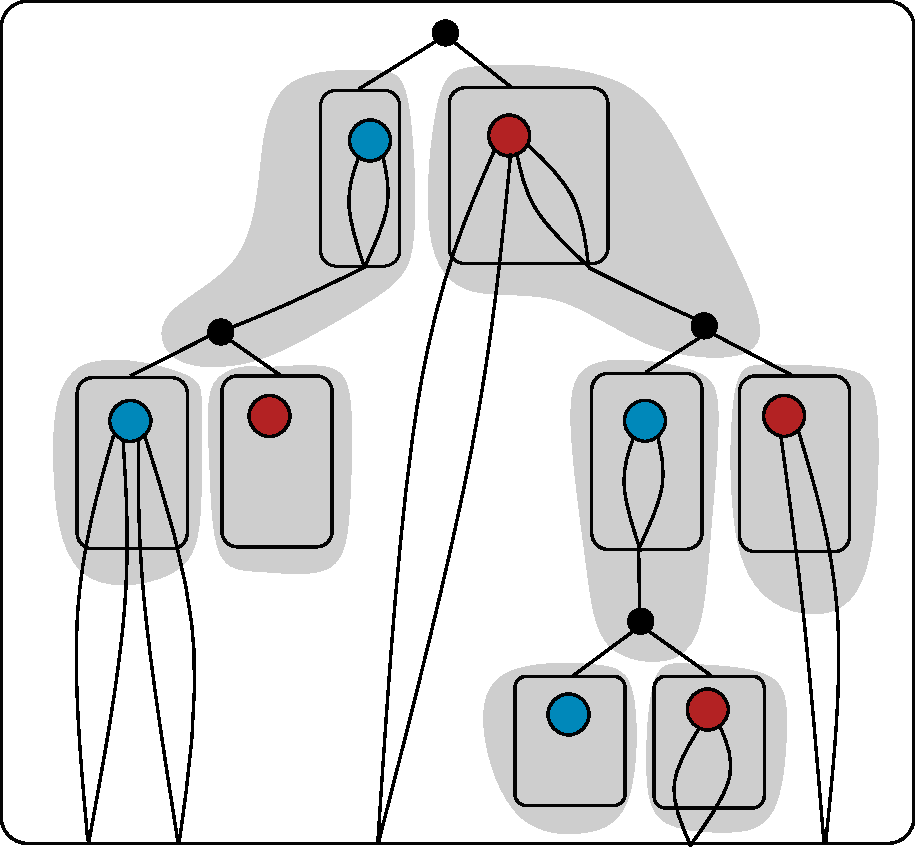
\includegraphics[scale=.3]{one-unfold3.pdf}
 \end{center}
 Note that we have two kind of factors: the first is a singleton and contains only a node labeled by $\ranked{k}$, the other kind of factors are those partial shallow terms $\ranked{(\reduce k \Sigma) * k}$. The idea now is to reflect this distinction in the type. That is to apply the function
 \begin{align*}
 \ranked{\tmonad \tmonad(k + \reduce k \Sigma) \to k. \tmonad ((\reduce k \Sigma)*k)}
 \end{align*}
 This function can be implemented easily using the decomposition function, the functions which maps every type to $\ranked{\bot}$ and mechanisms of raising errors. 
 \item Now the idea is to transform each node $\ranked{(\reduce k \Sigma)*k}$ into a $\rSigma$ one. We do so by transforming $\ranked{k}$ into $\ranked{1^k}$ (this function is basic since its domain is finite), then by applying the partial shallow unfold function of Example~\ref{ex:partial-shallow-unfold}, as illustrated by the following picture
   \begin{center}
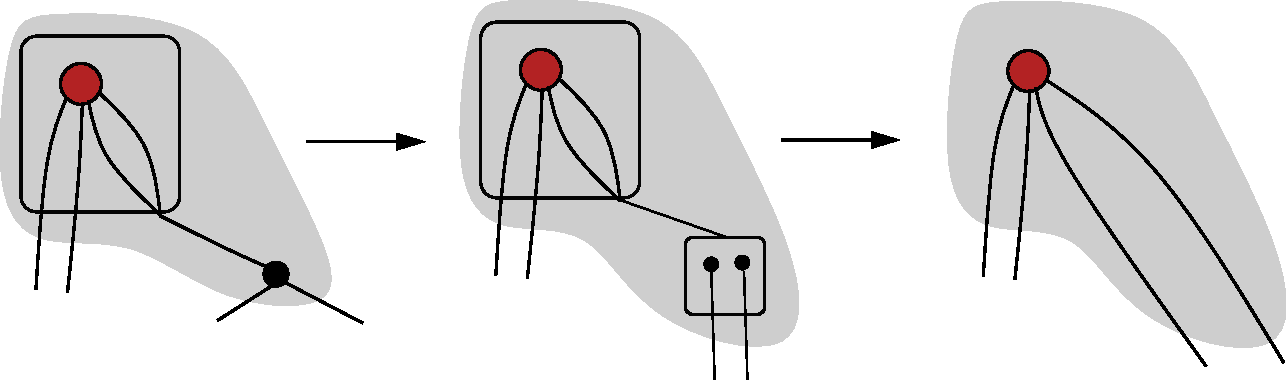
\includegraphics[scale=.3]{one-unfold4.pdf}
 \end{center}
 \end{itemize}
\end{proof}

\subsubsection{Term unfolding for $\alpha$-homogeneous inputs}
\label{subsec:alpha-homo-unfold}

For a monotone function 
\begin{align*}
\alpha: \set{1,\ldots,k} \to \set{1,\ldots,k}
\end{align*}
we say that a term $ t \in \tmonad \mati k \rSigma$ is $\alpha$-homogeneous if all internal branches have twist $\alpha$. This section is devoted to proving the following lemma. 

\begin{lemma}\label{lem:homo-twist}
    Let $k \in \set{1,2,\ldots}$ and let $\alpha : \set{1,\ldots,k} \to \set{1,\ldots,k}$ be a monotone function. There is a derivable operation 
    \begin{align*}
        \ranked{f : \tmonad \mati k \rSigma \to \mati k {(\tmonad \Sigma)} }
        \end{align*}      
which coincides with term unfolding for all inputs which are $\alpha$-homogeneous.
\end{lemma}

\begin{proof}
We proceed by induction on $k$. When $k=1$, the unfolding coincides with the basic distributivity function 
\begin{align*}
\ranked{ \tmonad \reduce 1 \Sigma \to {\reduce 1 \tmonad \Sigma}}
\end{align*}
Let us treat the inductive case. For that, we introduce a tool that will be useful to analyze the function $\alpha$. For a function $$\alpha: \set{1,\ldots,k} \to \set{1,\ldots,k}$$ define  \emph{its graph} as the directed graph whose set of vertices is $\set{1,\ldots,k}$, and which contains an edge $i\rightarrow j$ if $\alpha(i)=j$. Note that the out-degree of the nodes is $1.$

\medskip
In the proof of the inductive case, we distinguish two cases. The first one is when the graph of $\alpha$ is not weakly connected. In this case, by monotonicity of $\alpha$, we can find $m\in \set{1,k-1}$ such that $\alpha(\set{1,m})\subseteq\set{1,m}$ and $\alpha(\set{m+1,k})\subseteq\set{m+1,k}$. The idea is then to create two copies of the original tree: in the first one we keep only the first $m$ elements of the tensor product of each node, and in the second one we keep the last $k-m$ copies. Then we unfold these terms by applying the induction hypothesis, and  finally we gather them to obtain the  unfolding of the original term. 

%\smallskip
%To illustrate this case, we consider the following function $\alpha$, whose graph is shown below
%\begin{center}
%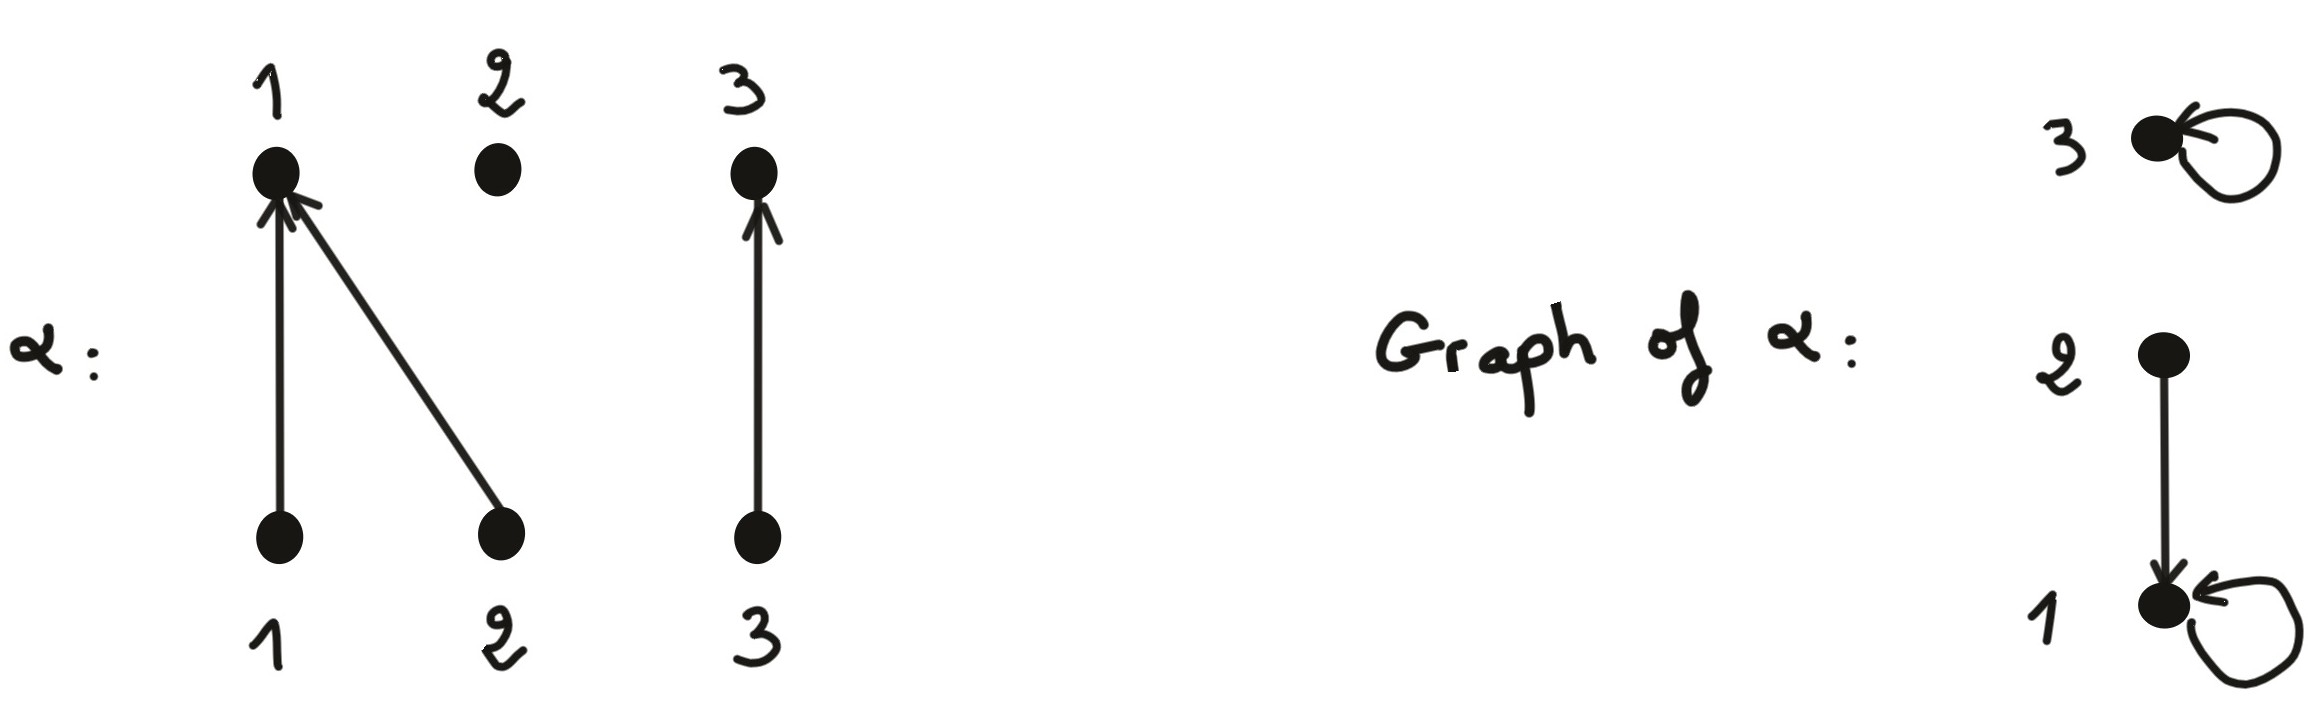
\includegraphics[scale=.07]{MyPic27.jpg}
%\end{center}
%The graph of $\alpha$ is not weakly connected: it contains two weakly connected components, $\set{1,2}$ and $\set{3}$.
%Consider the following $\alpha$-homogeneous terms $t$ of $\tmonad \mati k \rSigma$ which will be our running example in the not weakly connected case of the proof. We colored in blue the elements of the first weakly connected part of the graph of $\alpha$ and in green the second part.
%\begin{center}
%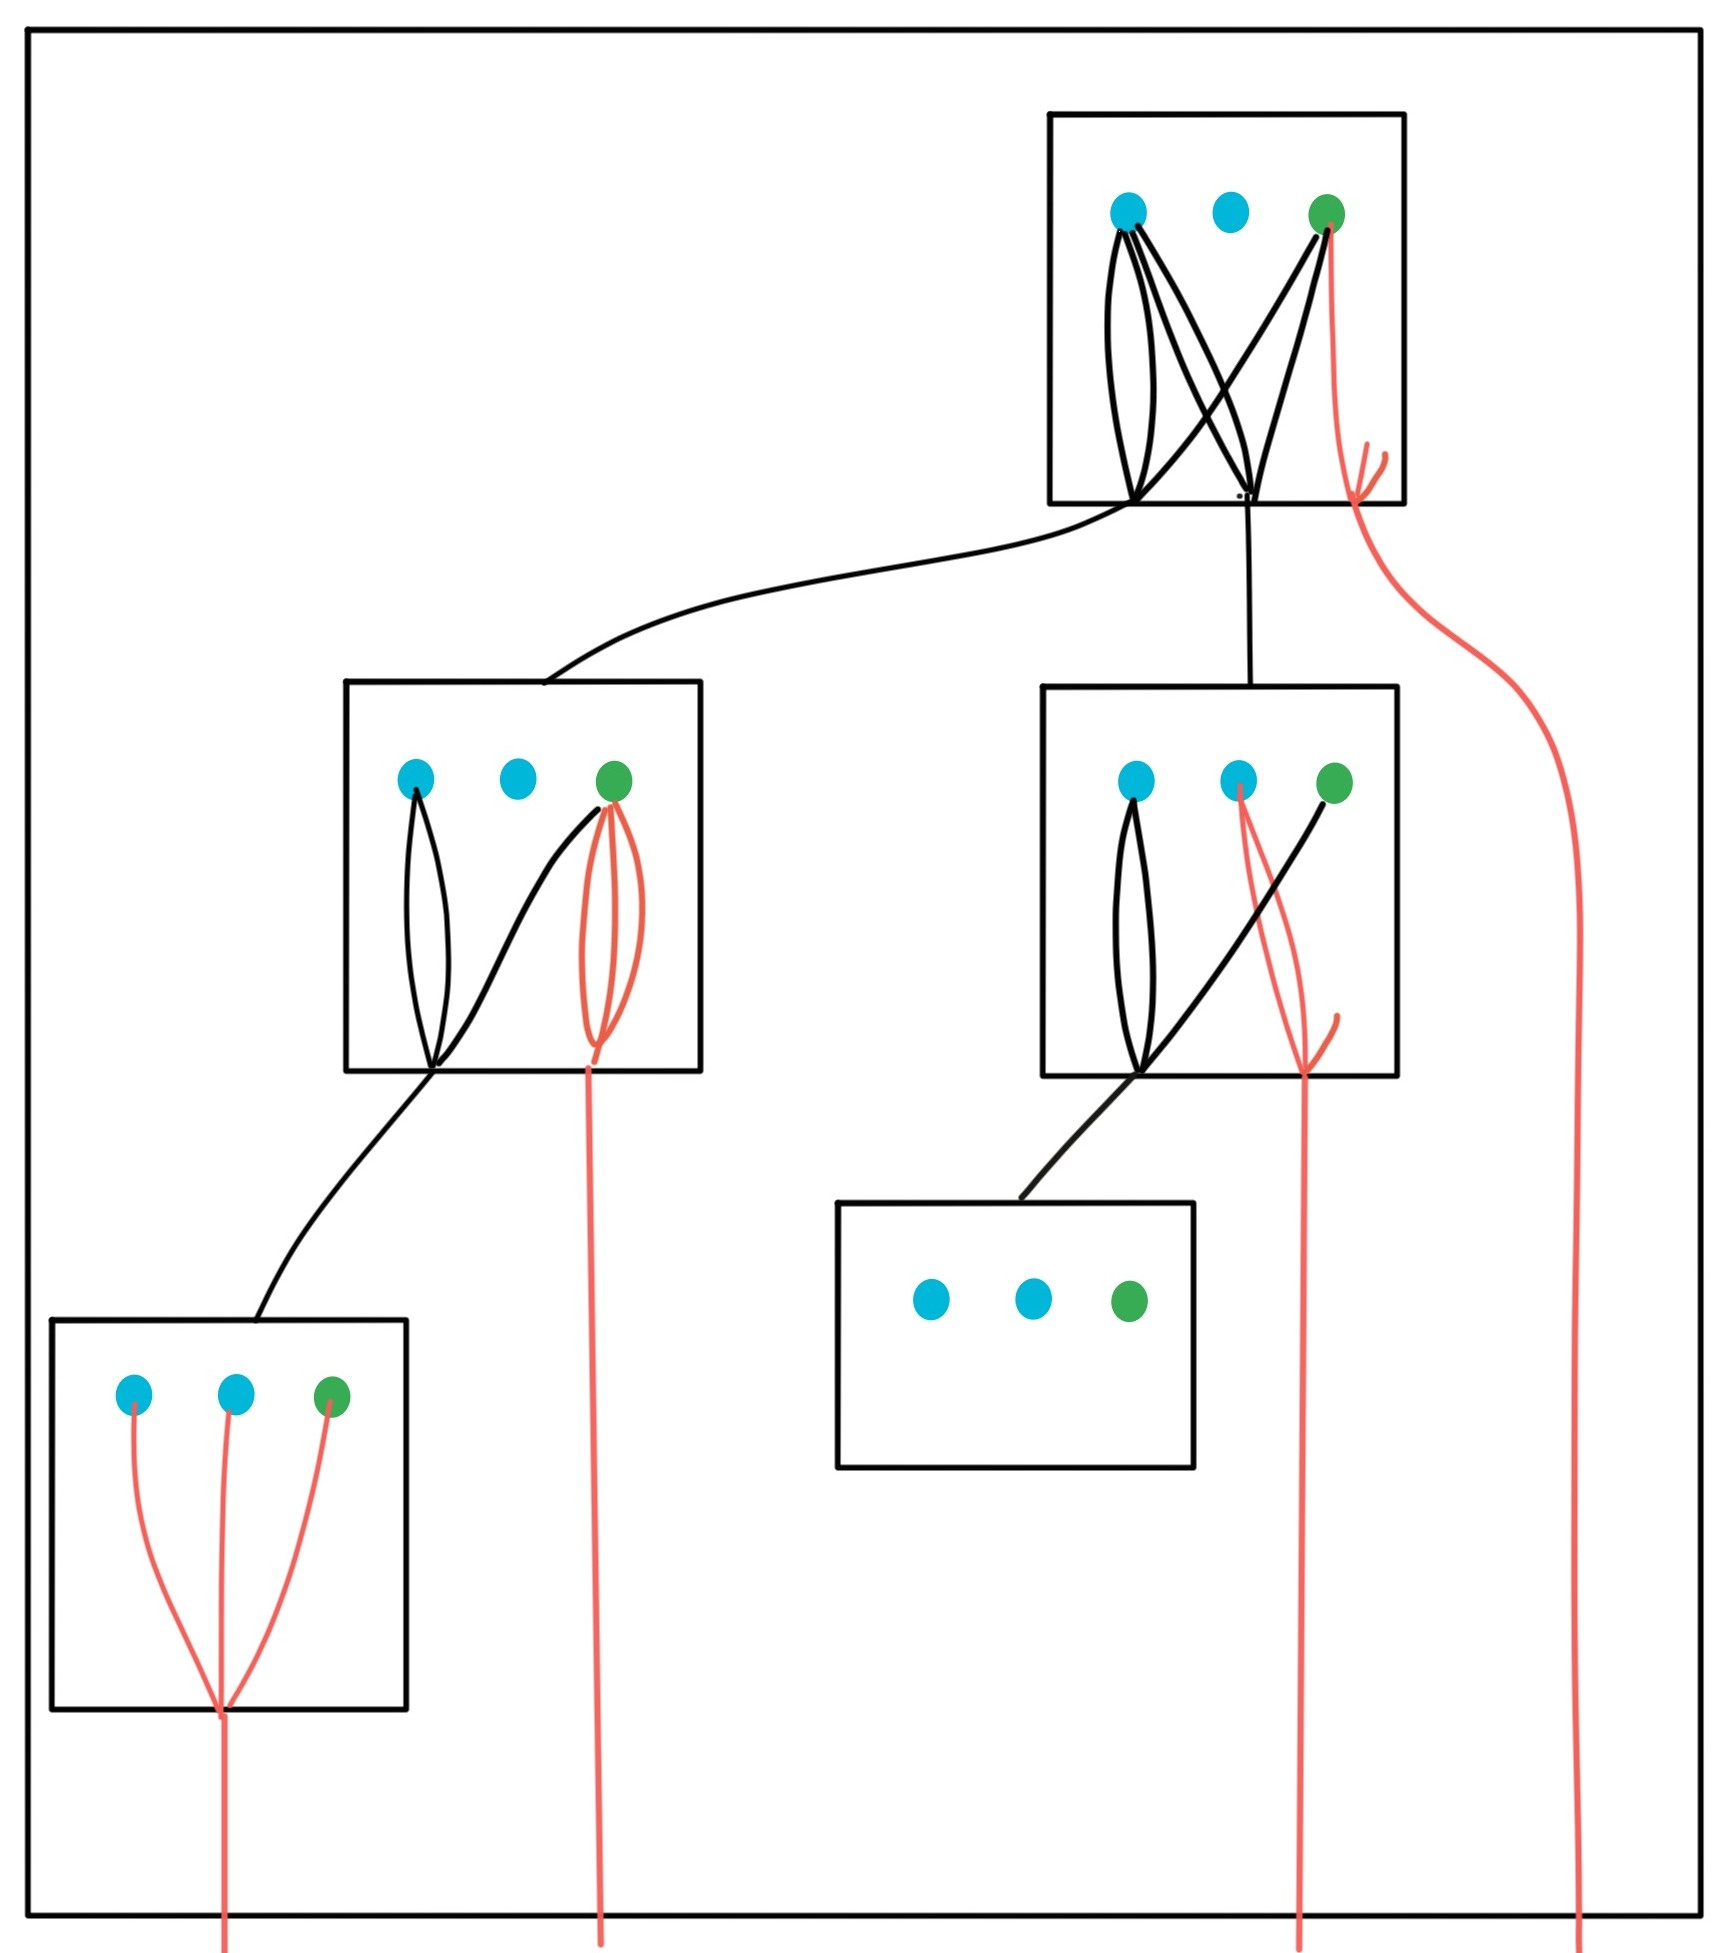
\includegraphics[scale=.07]{MyPic28.jpg}
%\end{center}
Let us now implement the ideas we discussed above. We start by unfolding the external twists, using the basic external unfold function. This way, the domain of every external twist  cannot be shared by the two disconnected components of the domain of $\alpha$.
%Our running example becomes like this:
%\begin{center}
%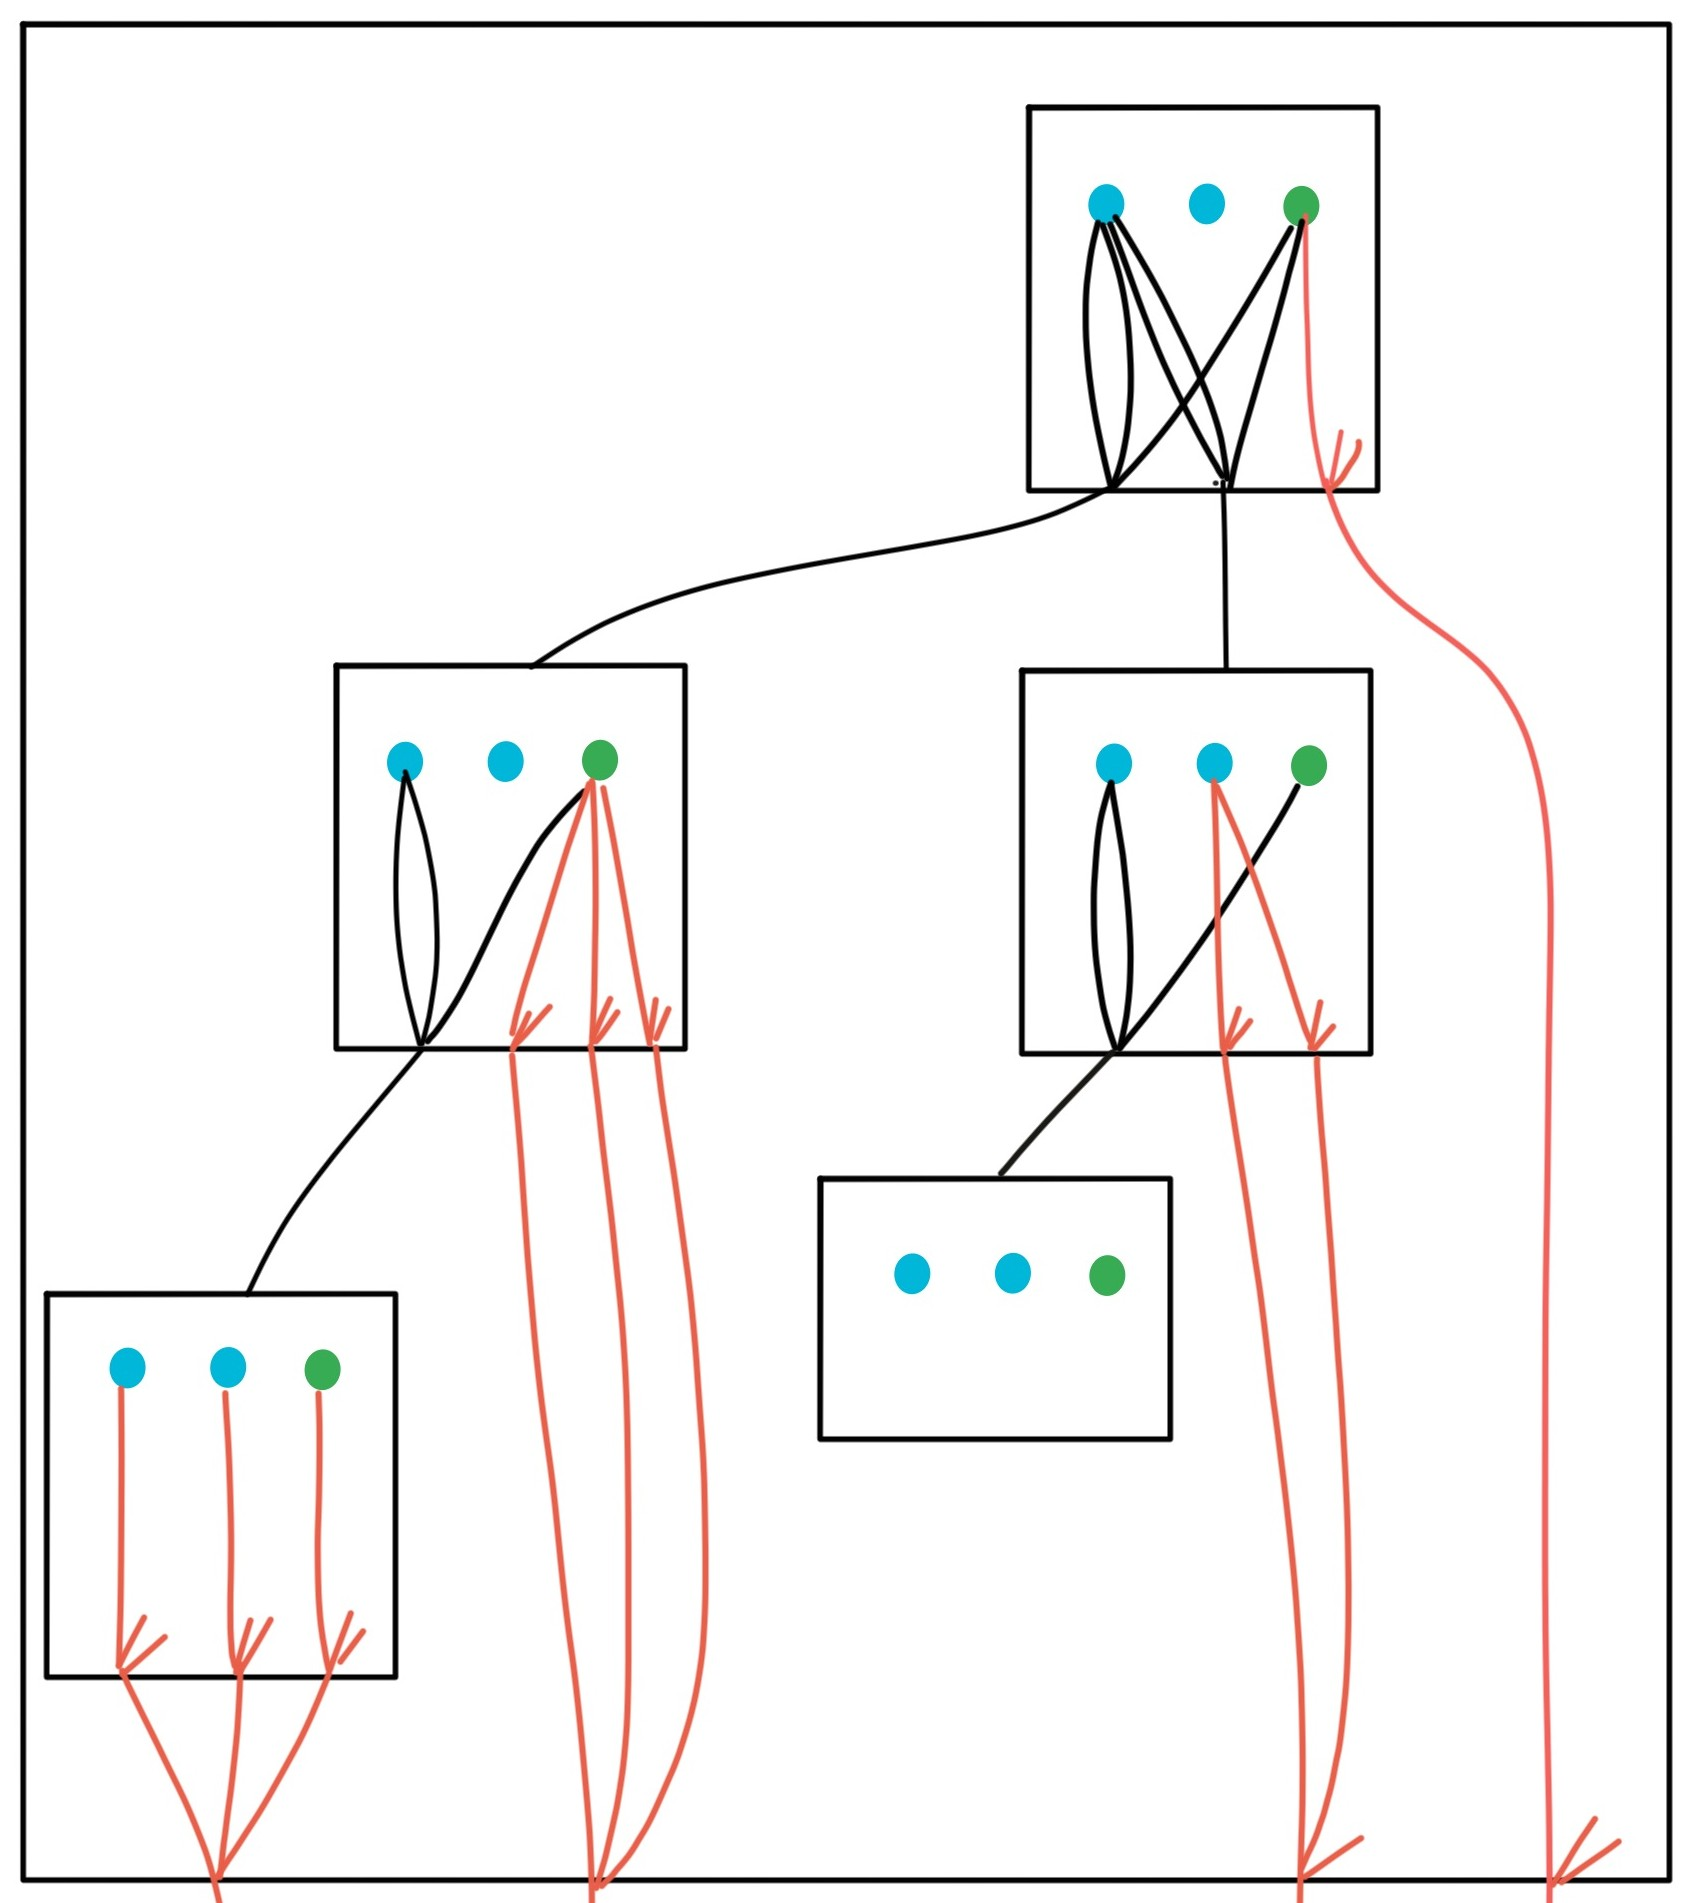
\includegraphics[scale=.07]{MyPic29.jpg}
%\end{center}
Then, we duplicate the input term using the basic function 
\begin{align*}
\ranked{\tmonad \mati k \Sigma\to \reduce 2 (\tmonad \mati k \Sigma\otimes \tmonad \mati k \Sigma)}
\end{align*}
To the first copy, we apply the function  
\begin{align*}
\ranked{f_1:\tmonad \mati k \Sigma \to \mati m {(\tmonad \Sigma)}}
\end{align*}
which keeps only the first $m$ elements of the tensor product, then applies the induction hypothesis to the obtained term.
To the second copy, we apply the function 
\begin{align*}
\ranked{f_2:\tmonad \mati k \Sigma \to \mati {k-m} {(\tmonad \Sigma)}}
\end{align*}
which keeps only the last $k-m$ elements of the tensor product, then applies the induction hypothesis to the obtained term.

%Here is the effect of the functions $f_1$ and $f_2$ on our example
%\begin{center}
%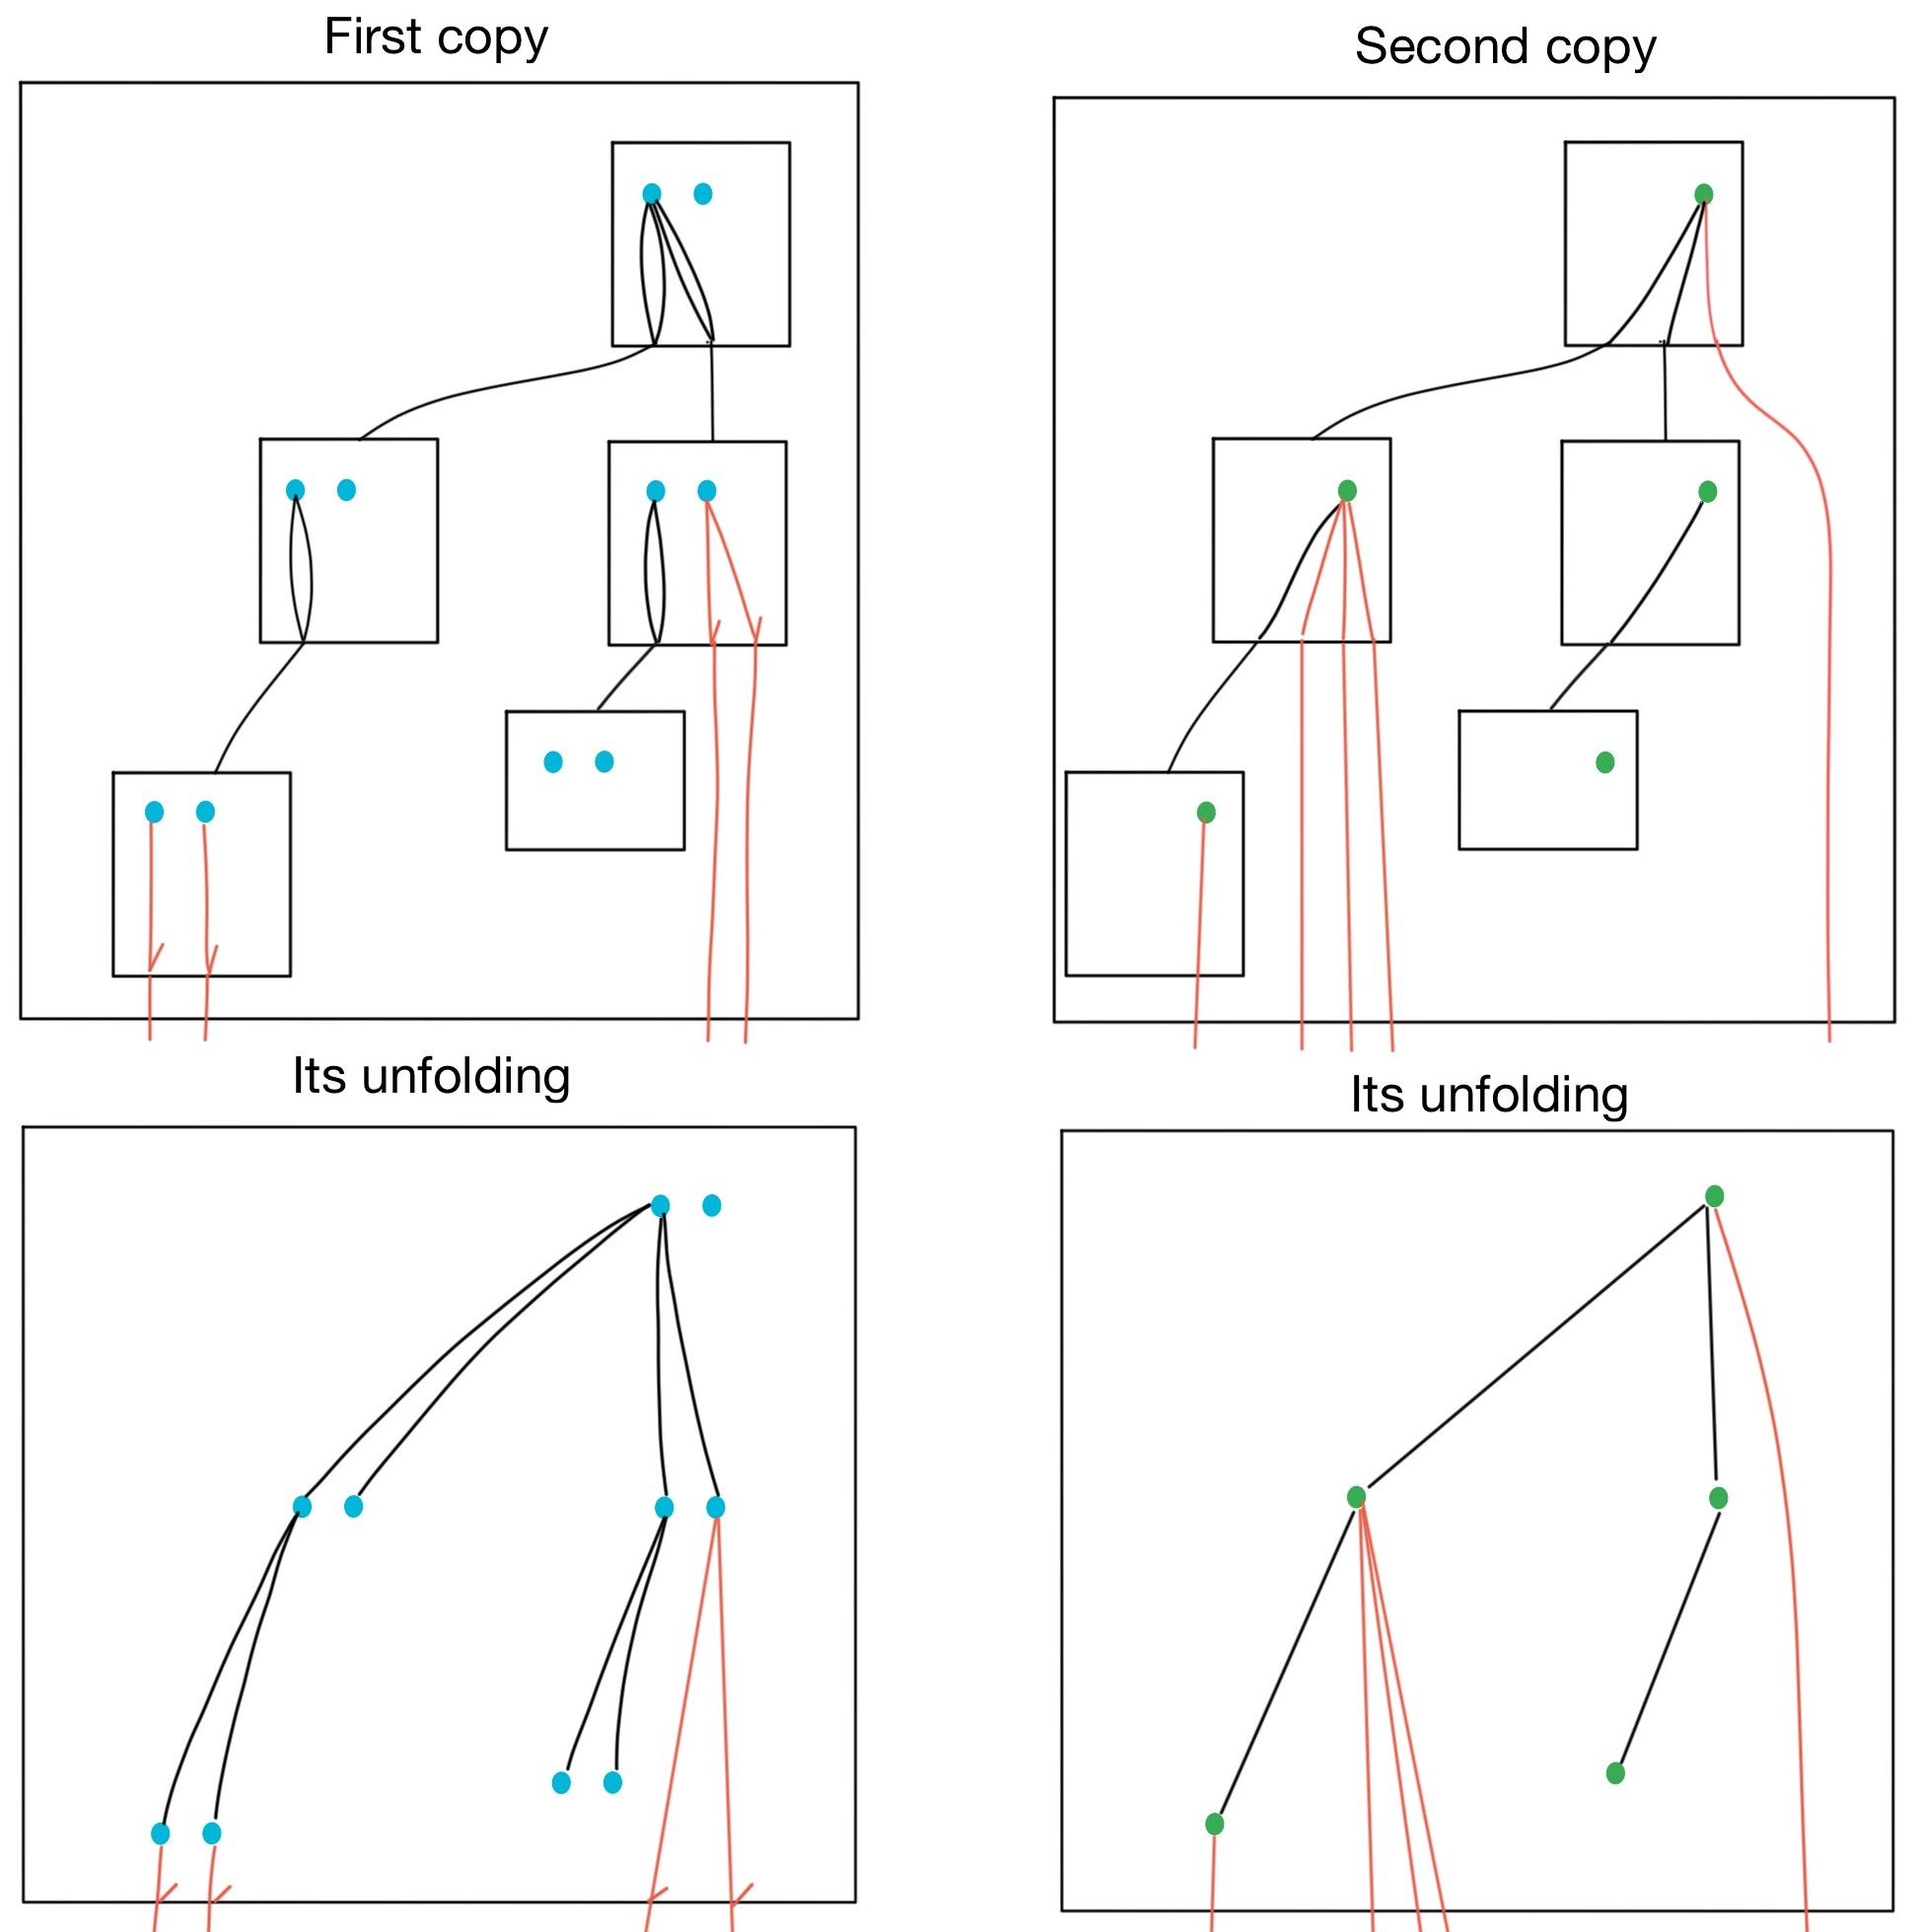
\includegraphics[scale=.15]{MyPic30.jpg}
%\end{center}
 The function $\ranked{f_1}$ can be derived using the tensor projection function, the merge of folds, then reducing the fold and finally invoking the induction hypothesis. 
%\begin{align*}
%\begin{prooftree}
%\Hypo{\overbrace{\ranked{\mati k \Sigma \to \reduce k \reduce 1 \Sigma^m}}^{\substack{\text{Lift the projection on the first}\\\text{$m$ elements of the tensor to $\reduce k$}}}}
%\Hypo{\overbrace{\ranked{\reduce k \reduccomponenetse 1 \Sigma^m \to \reduce k \Sigma^m}}^{\substack{\text{Merge the folds $\reduce k$ and $\reduce 1$}}}}
%\Hypo{\overbrace{\ranked{\reduce k \Sigma^m \to \mati m {(\Sigma\cdot (1+0))}}}^{\substack{\text{Adjust the degree of the fold}\\\text{to get a matrix power}}}}
%\Infer{3}[]{\ranked{\mati k \Sigma \to \mati m {(\Sigma\cdot (1+0))}}}
%\end{prooftree}
%\end{align*}


When we apply $f_1$ and $f_2$ to the two copies of the original term, we get a term of type 
\begin{align*}
\ranked{ \reduce 2 (\mati m {(\tmonad \Sigma)}\otimes  \mati {k-m} {(\tmonad\Sigma)})}
\end{align*}
%Now, we need to get the fold outside the tensor product. For that, we lift both $\ranked{\mati m {(\tmonad \Sigma)}}$ and $\ranked{\mati {k-m} {(\tmonad \Sigma)}}$ to $\ranked{\reduce k (\tmonad \Sigma)^m}$ and $\ranked{\reduce k (\tmonad \Sigma)^{k-m}}$ respectively. Then we commute the fold with the tensor product using the following basic function:
%\begin{align*}
%\ranked{\reduce k (\tmonad \Sigma)^m\otimes\reduce k (\tmonad \Sigma)^{k-m}\to \reduce k (\tmonad \Sigma)^k}
%\end{align*}
%Then we merge the two  folds $\reduce 2$ and $\reduce k$ into $\reduce {2k}$. After these operations, we get the desired term, but not with the desired type (the type we get is $\ranked{\reduce {2k} (\tmonad\Sigma)^k}$). To get the right type, which is $\ranked{\mati k {(\tmonad\Sigma)}}$, we apply the  function which reduces the degree of the fold
%\begin{align*}
%\ranked{\reduce {2k} (\tmonad \Sigma)^k \to \reduce {k} (\tmonad \Sigma)^k}
% \end{align*}
% The term we get for our example is the following, which is the unfolding of the original term
% \begin{center}
% 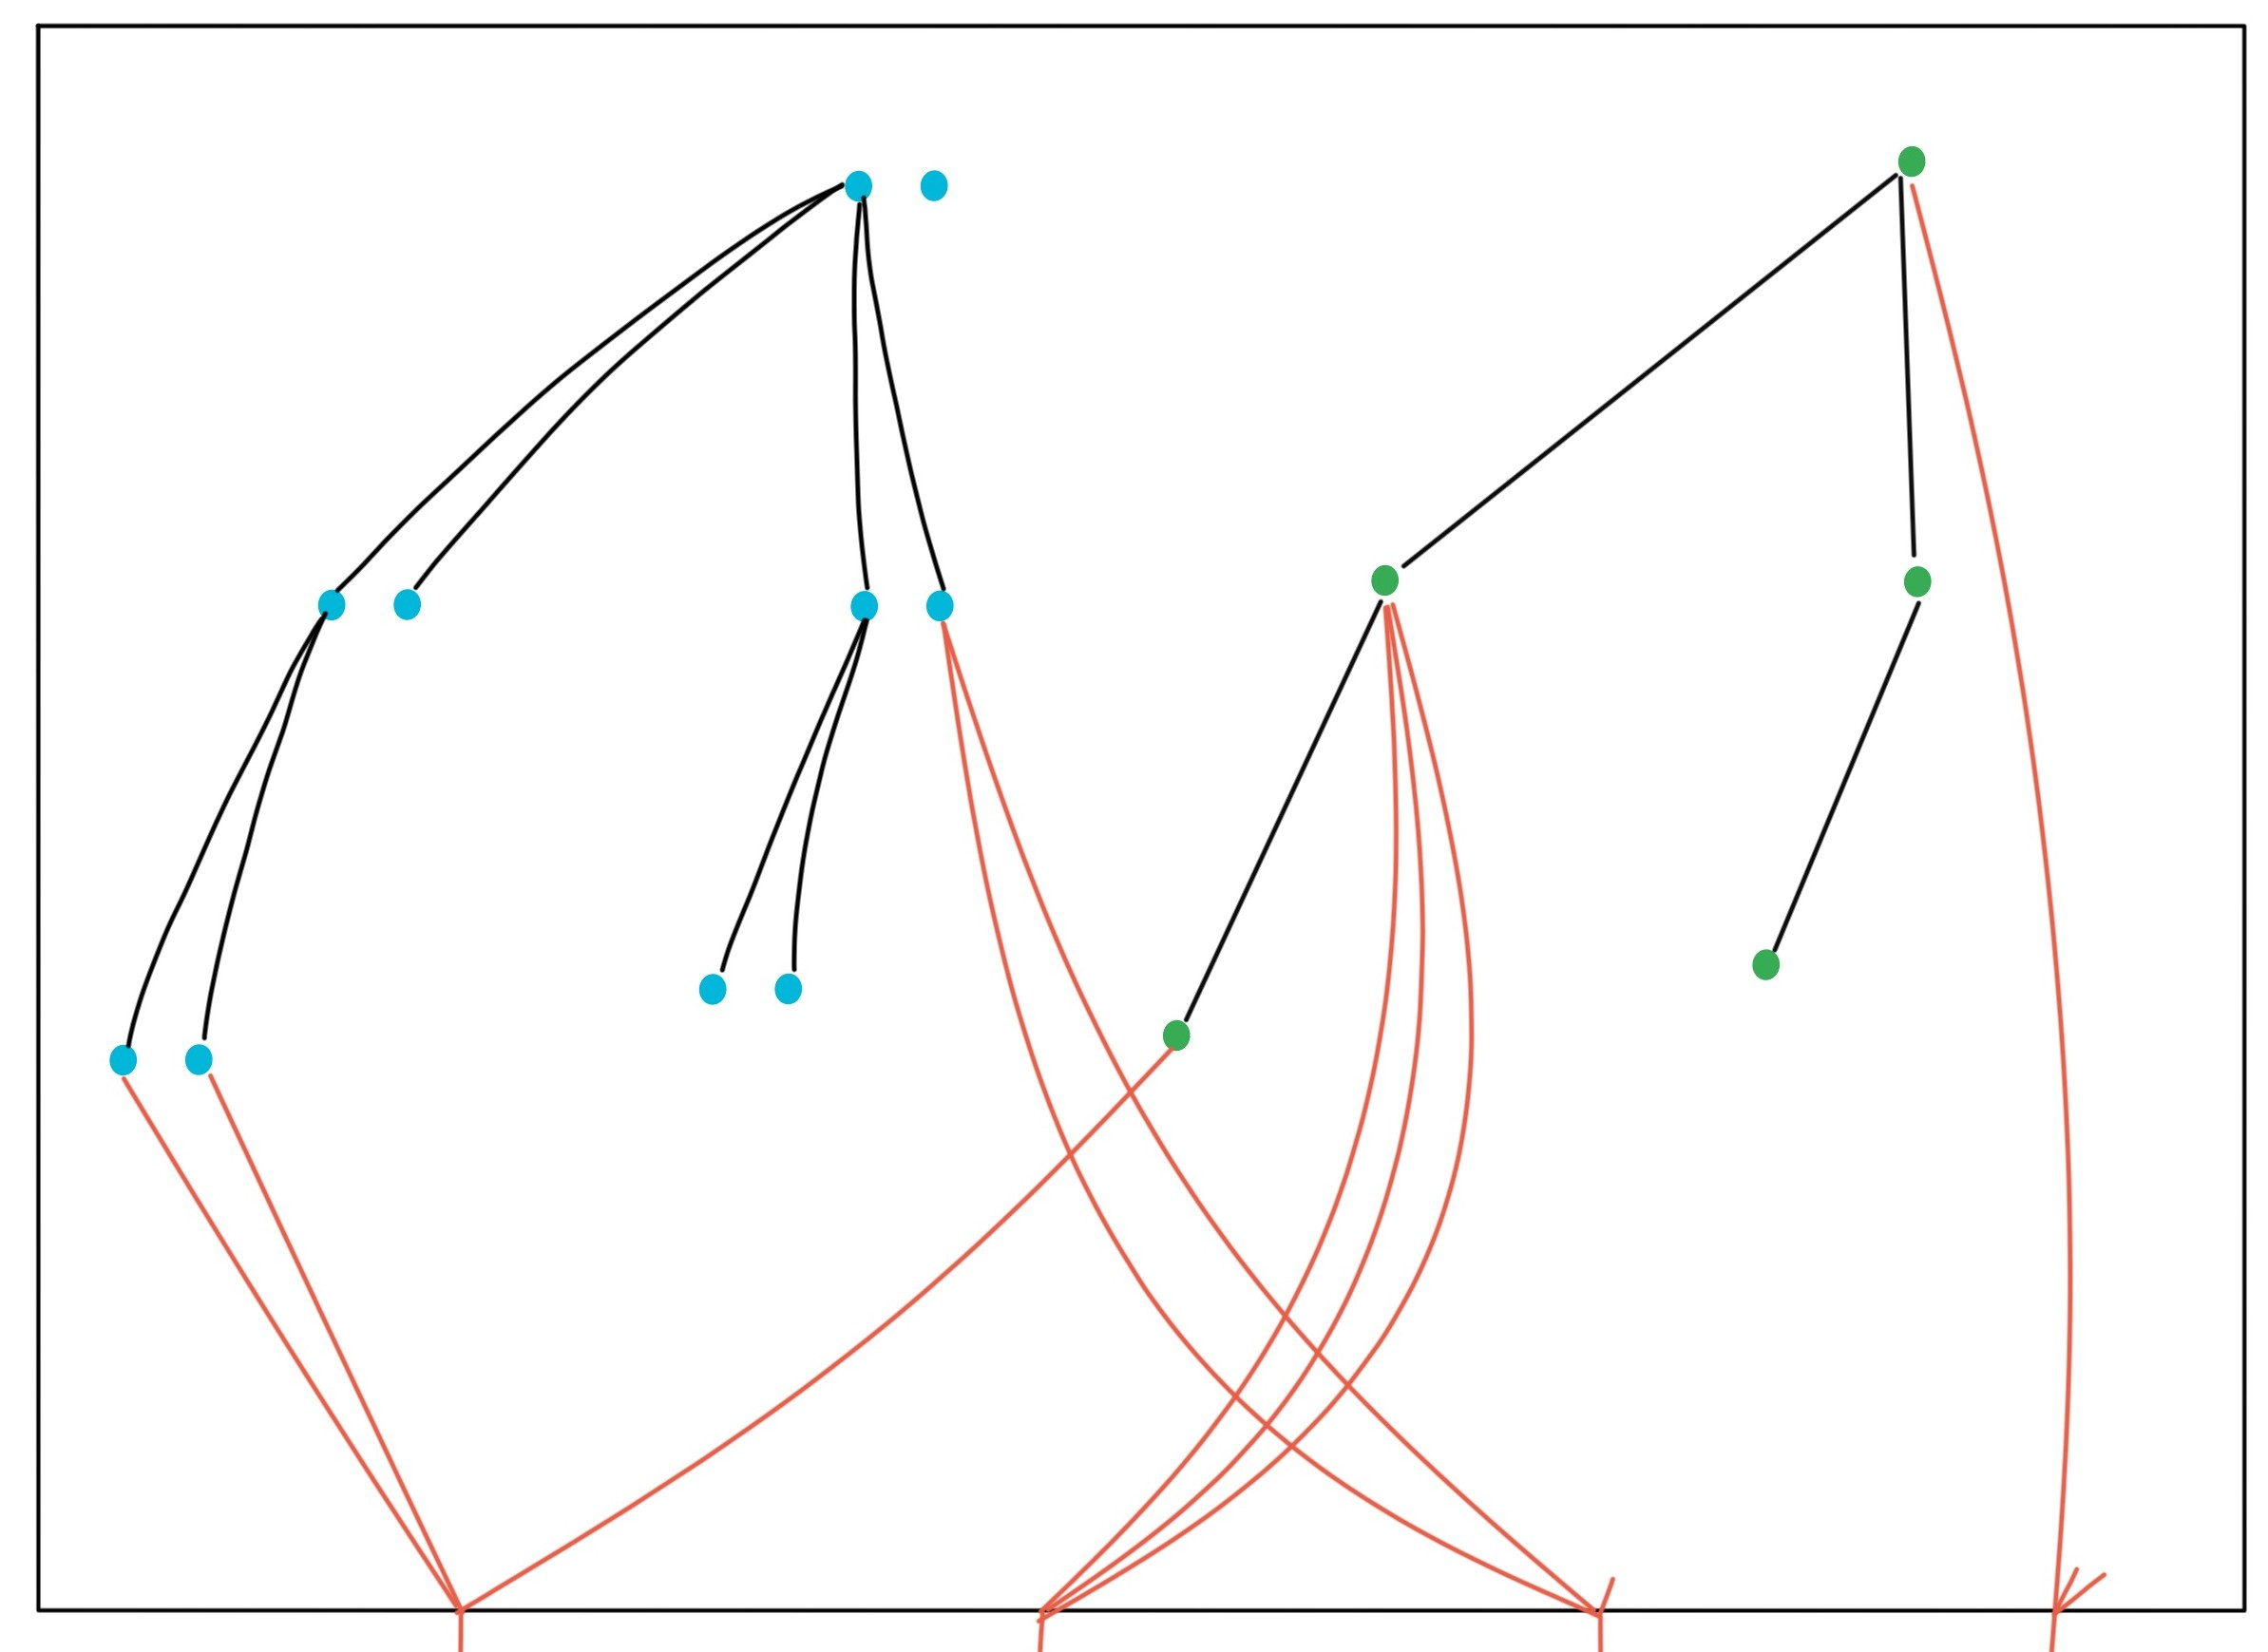
\includegraphics[scale=.08]{MyPic31.jpg}
% \end{center}
Apres une serie dinjections, de distributivites et de reductions de fold on obtien le resultat. Ptit truc: lorsqu'on reduit les fold, on a un bottom, qu'on fait remonter a la surface en utilisant une fonction d'error raising, a la fin on s'en debarasse dans le type en plongeant $\bot$ dans un arbre si on suppose que notre signature contient un element zeroaire et un element bianire. 
\medskip

Now consider the case where the graph of $\alpha$ is weakly connected. By monotonicity, we can show that either
\begin{align*}
\alpha^{-1}(1)=\emptyset\qquad\text{ or }\qquad\alpha^{-1}(k)=\emptyset
\end{align*}
By symmetry, we suppose wlog that $\alpha^{-1}(k)=\emptyset$. We suppose also that $\alpha(k)=k-1$, the general case can be treated in a similar way.
We consider as example the following function $\alpha$, whose graph, drawn below, is weakly connected
\begin{center}
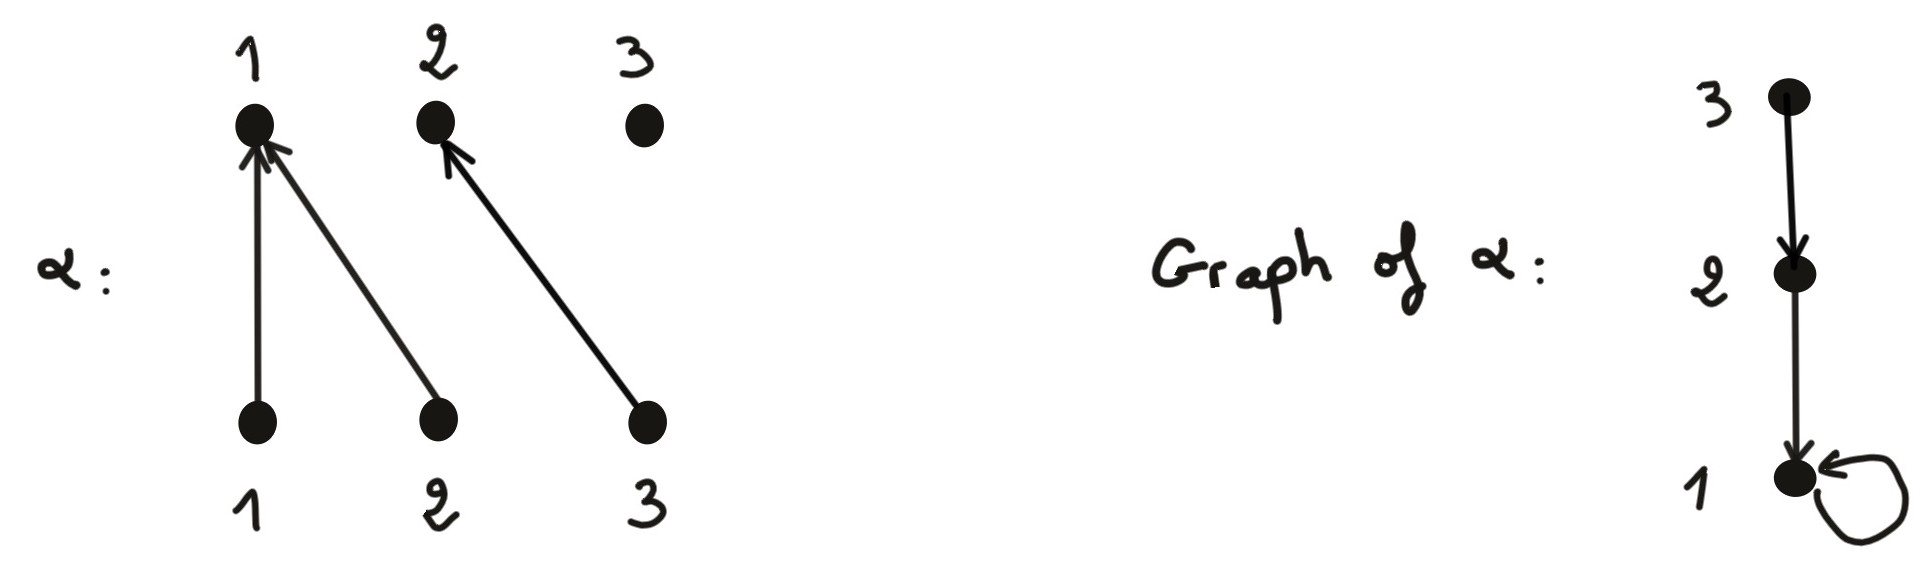
\includegraphics[scale=.1]{MyPic32.jpg}
\end{center}
we consider also the following $\alpha$-homogeneous term, where $\alpha$ is the function above, as running example for the weakly connected case. 

\end{proof}


\subsubsection{Term unfolding for homogeneous inputs}
\label{subsec:something-homo-unfold}
we say that a term $ t \in \tmonad \mati k \rSigma$ is homogeneous if for every two internal branches $b_1, b_2$ having twists $\alpha_1, \alpha_2$ respectively and such that $b_2$ is a child of $b_1$, we have that
\begin{align*}
\alpha_1\alpha_2=\alpha_1
\end{align*}

The rest of this section is devoted to proving the following lemma. 

\begin{lemma}\label{lem:homo-2-twist}
    Let $k \in \set{1,2,\ldots}$. There is a derivable operation 
    \begin{align*}
        \ranked{f : \tmonad \mati k \rSigma \to \mati k {(\tmonad \Sigma)} }
        \end{align*}      
which coincides with term unfolding for all inputs which are homogeneous.
\end{lemma}

\begin{lemma}
Let $\alpha:[1,k]\to [1,k]$ and $\beta:[1,k]\to [1,k]$ be two monotone functions such that
\begin{align*}
\alpha\beta=\alpha.
\end{align*}
 If the graph of $\alpha$ is not weakly connected, then so is the graph of $\beta$. Moreover, if $m\in \set{1,\dots, k}$ is such that 
\begin{align*}
\alpha[1,m] \subseteq [1,m]  \text{ and } 
\alpha[m+1,k]\subseteq [m+1,k]
\end{align*}
then we have also 
\begin{align*}
\beta[1,m]\subseteq [1,m] \text{ and }
\beta[m+1,k]\subseteq [m+1,k]
\end{align*}

 If the graphs of $\alpha$ and $\beta$ are both weakly connected, then the image of $\alpha$ and the image of $\beta$ are both singletons.
\end{lemma}

\begin{proof}[Proof of Lemma~\ref{lem:homo-2-twist}]

\end{proof}
